
\chapter{ingress controller}
%\section{ingress controller}
\label{appendix:ingress_controller}

\begin{lstlisting}[
    basicstyle=\footnotesize,
    breaklines=true,
    postbreak=\mbox{\textcolor{red}{$\hookrightarrow$}\space},
  ]
package main

import (
	"log"
	"net/http"
	"os"
	"syscall"
	"os/exec"
	"strings"
	"text/template"
	"github.com/spf13/pflag"
	api "k8s.io/client-go/pkg/api/v1"
	nginxconfig "k8s.io/ingress/controllers/nginx/pkg/config"
	"k8s.io/ingress/core/pkg/ingress"
	"k8s.io/ingress/core/pkg/ingress/controller"
	"k8s.io/ingress/core/pkg/ingress/defaults"
)

var cmd = exec.Command("keepalived", "-nCDlf", "/etc/keepalived/ipvs.conf")

func main() {
	ipvs := newIPVSController()
	ic := controller.NewIngressController(ipvs)
	cmd.Stdout = os.Stdout
	cmd.Stderr = os.Stderr
	cmd.Start()
	defer func() {
		log.Printf("Shutting down ingress controller...")
		ic.Stop()
	}()
	ic.Start()
}

func newIPVSController() ingress.Controller {
	return &IPVSController{}
}

type IPVSController struct{}

func (ipvs IPVSController) SetConfig(cfgMap *api.ConfigMap) {
	log.Printf("Config map %+v", cfgMap)
}

func (ipvs IPVSController) Reload(data []byte) ([]byte, bool, error) {
	cmd.Process.Signal(syscall.SIGHUP)
	out, err := exec.Command("echo", string(data)).CombinedOutput()
	if err != nil {
		return out, false, err
	}
	log.Printf("Issue kill to keepalived. Reloaded new config %s", out)
	return out, true, err
}

func (ipvs IPVSController) OnUpdate(updatePayload ingress.Configuration) ([]byte, error) {
	log.Printf("Received OnUpdate notification")
	for _, b := range updatePayload.Backends {
		type ep struct{
			Address,Port string
		}
		eps := []ep{}
		for _, e := range b.Endpoints {
			eps = append(eps, ep{Address: e.Address, Port: e.Port})
		}

		for _, a := range eps {
		log.Printf("Endpoint %v:%v added to %v:%v.", a.Address, a.Port, b.Name, b.Port)
		}

		if b.Name == "upstream-default-backend" {
			continue
		}
		cnf := []string{"/etc/keepalived/ipvs.d/" , b.Name , ".conf"}
		w, err := os.Create(strings.Join(cnf, ""))
		if err != nil {
			return []byte("Ooops"), err
		}
		tpl := template.Must(template.ParseFiles("ipvs.conf.tmpl"))
		tpl.Execute(w, eps)
		w.Close()
	}
	
	return []byte("hello"), nil
}

func (ipvs IPVSController) BackendDefaults() defaults.Backend {
	// Just adopt nginx's default backend config
	return nginxconfig.NewDefault().Backend
}

func (ipvs IPVSController) Name() string {
	return "IPVS Controller"
}

func (ipvs IPVSController) Check(_ *http.Request) error {
	return nil
}

func (ipvs IPVSController) Info() *ingress.BackendInfo {
	return &ingress.BackendInfo{
		Name:       "dummy",
		Release:    "0.0.0",
		Build:      "git-00000000",
		Repository: "git://foo.bar.com",
	}
}

func (ipvs IPVSController) OverrideFlags(*pflag.FlagSet) {
}

func (ipvs IPVSController) SetListers(lister ingress.StoreLister) {
}

func (ipvs IPVSController) DefaultIngressClass() string {
	return "ipvs"
}
\end{lstlisting}

\chapter{ECMP settings}
\section{Exabgp configuration on the load balancer container.}
\label{appendix:exabgp_config}

{\bf\normalsize exabgp.conf:}
\begin{verbatim}
neighbor 10.0.0.109 {
 description "peer1";
 router-id 172.16.20.2;
 local-address 172.16.20.2;
 local-as 65021;
 peer-as 65021;
 hold-time 1800;
   static {
     route 10.1.1.0/24 next-hop 10.0.0.106;
   }
}
\end{verbatim}

\section{Gobgpd configuration on the route reflector.}
\label{appendix:route_reflector_config}

{\bf\normalsize gobgp.conf:}
\begin{verbatim}
global:
  config:
    as: 65021
    router-id: 10.0.0.109
    local-address-list:
    - 0.0.0.0 # ipv4 only
  use-multiple-paths:
    config:
      enabled: true

peer-groups:
  - config:
      peer-group-name: k8s
      peer-as: 65021
    afi-safis:
      - config:
          afi-safi-name: ipv4-unicast

dynamic-neighbors:
  - config:
      prefix: 172.16.0.0/16
      peer-group: k8s

neighbors:
  - config:
      neighbor-address: 10.0.0.110
      peer-as: 65021
    route-reflector:
      config:
        route-reflector-client: true
        route-reflector-cluster-id: 10.0.0.109
    add-paths: 
      config:
        send-max: 255
        receive: true

\end{verbatim}

\section{Gobgpd and zebra configurations on the router.}

{\bf\normalsize gobgp.conf:}
\begin{verbatim}
global:
  config:
    as: 65021
    router-id: 10.0.0.110
    local-address-list:
    - 0.0.0.0

  use-multiple-paths:
    config:
      enabled: true

neighbors:
    - config:
        neighbor-address: 10.0.0.109
        peer-as: 65021
      add-paths:
        config:
          receive: true

zebra:
  config:
    enabled: true
    url: unix:/run/quagga/zserv.api
    version: 3
    redistribute-route-type-list: 
      - static

\end{verbatim}
\label{appendix:router_config}
%
{\bf\normalsize zebra.conf:}
\begin{verbatim}
hostname Router
log file /var/log/zebra.log
\end{verbatim}

%\caption{Example of zebra config on the router.}
%\label{fig:zebra_config_router}

\chapter{Analysis of the performance limit}
\label{appendix:performance_limit}

The maximum throghput in this series of experiment is roughly, 190k[req/sec] for both ipvs an the iptables DNAT.
At first, it was not clear what caused this limit.
The author analyzed the kind of packets that flows during the experiment using tcpdump\cite{jacobson1989tcpdump} as follows;
1) A wrk worker opens multiple connections and sends out http request to the web servers. The number of connections is determined by the command-line option, eg. 800/40 = 20 connection in the case of command-line in Table~\ref{tab:bench_example}. The worker sends out 100 requests to the web server within each connection, and closes it either if all of the responses are recieved or time out occurs.
2) As in seen in Listing~\ref{list:tcpdump}, tcp options were mss(4 byte), sack(2 byte), ts(10 byte), nop(1 byte) and wscale(3 byte), for SYN packets. For other packets, tcp options were, nop(1 byte), nop(1 byte) and ts(10 byte).
3) The author classified the types of packes and counted the number of each type in a single connection, which is 100 http requests. Table~\ref{tab:request_data_size},\ref{tab:response_data_size},\ref{tab:header_size} summarize the data size of 100 request, including TCP headr, IP header, Ether header and overheads. 
From this analysis, it was found that per each HTTP request and response,
request data with the size of 227.68[byte] and response data with the data(http content)+437.68[byte] were being sent.   

Since the node for load balancer recives and transmits both request and response packets using single network interface, each 1Gbps half duplex of full duplex must accomodate request and response data size.
Therefore the theoretical maximum throughput can be expressed as; \\
throughput[req/sec] = band width[byte/sec]/(request + response) \\
= 1e9/8/(data+665.36)

Figure~\ref{fig:performance_limit} shows plot of theoretical maximum throughput 1Gbps ethernet together with actual benchmark results.
Since experimnetal results agrees well with theory, the author concludes that when \enquote{RPS = on}, ipvs performance limit is due to the 1Gbps bandwidth.

\begin{lstlisting}[
    backgroundcolor = \color{mygray},
    basicstyle=\footnotesize,
    breaklines=true,
    numbers=left,
    %    postbreak=\mbox{\textcolor{red}{$\hookrightarrow$}\space},
    caption={An example of the tcpdump output},
    captionpos=b,
    label={list:tcpdump}
  ]
  curl -s  http://172.16.72.2:8888/1000
  tcpdmup(response):

  03:09:27.968942 IP 172.16.72.2.8888 > 192.168.0.112.60142:
  Flags [S.], seq 2317920646, ack 648140715, win 28960, options [mss 1460,sackOK,TS val 2274012282 ecr 2324675546,nop,wscale 8], length 0
  03:09:27.969685 IP 172.16.72.2.8888 > 192.168.0.112.60142:
  Flags [.], ack 85, win 114, options [nop,nop,TS val 2274012282 ecr 2324675546], length 0
  03:09:27.969945 IP 172.16.72.2.8888 > 192.168.0.112.60142:
  Flags [P.], seq 1:255, ack 85, win 114, options [nop,nop,TS val 2274012282 ecr 2324675546], length 254
  03:09:27.969948 IP 172.16.72.2.8888 > 192.168.0.112.60142:
  Flags [P.], seq 255:1255, ack 85, win 114, options [nop,nop,TS val 2274012282 ecr 2324675546], length 1000
  03:09:27.970846 IP 172.16.72.2.8888 > 192.168.0.112.60142:
  Flags [F.], seq 1255, ack 86, win 114, options [nop,nop,TS val 2274012282 ecr 2324675547], length 0
\end{lstlisting}

\begin{table}[h]
\centering
  \begin{tabular}{|l|r|r|r|r|}
    \hline
%    \multicolumn{5}{|l|}{Data size in 100 HTTP requests.} \\ \hline
    Type of Packet & \multicolumn{1}{l|}{Payload {[}byte{]}} & \multicolumn{1}{l|}{Header {[}byte{]}} & \multicolumn{1}{l|}{Count} & \multicolumn{1}{l|}{Total {[}byte{]}} \\ \hline
    SYN & 0 & 98 & 1 & 98 \\ \hline
    ACK & 0 & 90 & 102 & 9,180 \\ \hline
    Push(GET) & 44 & 90 & 100 & 13,400 \\ \hline
    FIN+ACK & 0 & 90 & 1 & 90 \\ \hline
    \multicolumn{3}{|l|}{Total} & \multicolumn{2}{r|}{22,768} \\ \hline
  \end{tabular}
  \caption{Request data size for 100 HTTP requests in wrk measurement.}
  \label{tab:request_data_size}
%% \end{table}

  \vspace{1cm}
  
%% \begin{table}[h]
\centering
  \begin{tabular}{|l|r|r|r|r|}
    \hline
%    \multicolumn{5}{|l|}{Response Data size for 100 HTTP requests in wrk measurement.} \\ \hline
    Type of Packet & \multicolumn{1}{l|}{Payload {[}byte{]}} & \multicolumn{1}{l|}{Header {[}byte{]}} & \multicolumn{1}{l|}{Count} & \multicolumn{1}{l|}{Total {[}byte{]}} \\ \hline
    SYN+ACK & 0 & 98 & 1 & 98 \\ \hline
    ACK & 0 & 90 & 2 & 180 \\ \hline
    Push(GET) & 254 & 90 & 100 & 34,400 \\ \hline
    Push(DATA) & data & 90 & 100 & 100x(data+90) \\ \hline
    FIN+ACK & 0 & 90 & 1 & 90 \\ \hline
    \multicolumn{3}{|l|}{Total} & \multicolumn{2}{r|}{100x(data+90)+34,768} \\ \hline
  \end{tabular}
  \caption{Response data size for 100 HTTP requests in wrk measurement.}
  \label{tab:response_data_size}
\end{table}

\begin{table}[h]
\begin{center}
  \begin{tabular}{|l|r|r|}
    \hline
    Type of field & \multicolumn{1}{l|}{SYN} & \multicolumn{1}{l|}{\begin{tabular}[c]{@{}l@{}}ACK, SYN+ACK,\\ FIN+ACK, PUSH\end{tabular}} \\ \hline
    preamble & 8 & 8 \\ \hline
    ether header & 14 & 14 \\ \hline
    ip header & 20 & 20 \\ \hline
    tcp header & 20 + 20(tcp options) & 20 + 12(tcp options) \\ \hline
    fcs & 4 & 4 \\ \hline
    inter frame gap & 12 & 12 \\ \hline
    Total [byte] & 98 & 90 \\ \hline
  \end{tabular}
  \caption{Header sizes of TCP/IP packet in Ethernet frame.}
  \label{tab:header_size}
\end{center}
\end{table}


\chapter{VRRP}
\section{VRRP}\label{sec:vrrp}

\begin{figure}[tb]
\centering
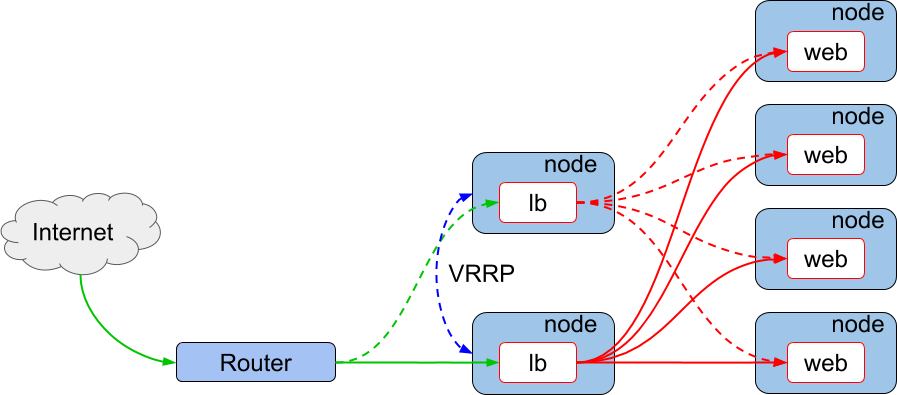
\includegraphics[width=0.8\columnwidth]{Figs/vrrp.png}
\caption{
  An alternative redundant load balancer architecture using VRRP.
}
\centering\parbox[c]{0.9\columnwidth}{
  The traffic from the internet is forwarded by the upstream router to a active lb node and then distributed by the lb pods to web pods using Linux kernel's ipvs.
  The active lb pod is selected using VRRP protocol.
}
\label{fig:vrrp}
\end{figure}

Fig.~\ref{fig:vrrp} shows an alternative redundancy setup using the VRRP protocol that was first considered by the authors, but did not turn out to be preferable.
In the case of VRRP, the load balancer container needs to run in the node net namespace for the following two reasons.
1) When fail over occurs, the new master sends gratuitous Address Resolution Packets(ARP) packets to update the ARP cache of the upstream router and Forwarding Data Base(FDB) of layer 2 swicthes during the transition.
Such gratuitous ARP packets should consist of the virtual IP address shared by the load balancers and the MAC address of the node where the new master load balancer is running.
Programs that send out gratuitous ARP with node MAC address should be in the node net namespace.
%
2) Furthermore, the active load balancer sends out periodic advertisement using UDP multicast packet to inform existence of itself.
The load balancer in backup state stays calm unless the VRRP advertisement stops for a specified duration of time.
The UDP multicast is often unsupported in overlay network used by container cluster environment, and hence the load balancer needs to be able to use the node net namespace.
%
Running containers in the node net namespace loses the whole point of containerization, i.e., they share the node network without separation.
This requires the users' additional efforts to avoid conflict in VRRP configuration for multiple services.
%

VRRP programs also support unicast advertisement by specifying IP addresses of peer load balancers before it starts.
However, container cluster management system randomly assign IP addresses of containers when it launches them, and it is impossible to know peer IPs in advance. 
Therefore the unicast mode is not feasible in container cluster environment.

The other drawback compared with the ECMP case is that the redundancy of VRRP is provided in Active-Backup manner.
This means that a single software load balancer limits the overall performance of the entire container cluster.
Therefore we believe the ECMP redundancy is better than VRRP in our use cases.

